
% Default to the notebook output style

    


% Inherit from the specified cell style.




    
\documentclass[11pt]{article}

    
    
    \usepackage[T1]{fontenc}
    % Nicer default font than Computer Modern for most use cases
    \usepackage{palatino}

    % Basic figure setup, for now with no caption control since it's done
    % automatically by Pandoc (which extracts ![](path) syntax from Markdown).
    \usepackage{graphicx}
    % We will generate all images so they have a width \maxwidth. This means
    % that they will get their normal width if they fit onto the page, but
    % are scaled down if they would overflow the margins.
    \makeatletter
    \def\maxwidth{\ifdim\Gin@nat@width>\linewidth\linewidth
    \else\Gin@nat@width\fi}
    \makeatother
    \let\Oldincludegraphics\includegraphics
    % Set max figure width to be 80% of text width, for now hardcoded.
    \renewcommand{\includegraphics}[1]{\Oldincludegraphics[width=.8\maxwidth]{#1}}
    % Ensure that by default, figures have no caption (until we provide a
    % proper Figure object with a Caption API and a way to capture that
    % in the conversion process - todo).
    \usepackage{caption}
    \DeclareCaptionLabelFormat{nolabel}{}
    \captionsetup{labelformat=nolabel}

    \usepackage{adjustbox} % Used to constrain images to a maximum size 
    \usepackage{xcolor} % Allow colors to be defined
    \usepackage{enumerate} % Needed for markdown enumerations to work
    \usepackage{geometry} % Used to adjust the document margins
    \usepackage{amsmath} % Equations
    \usepackage{amssymb} % Equations
    \usepackage{textcomp} % defines textquotesingle
    % Hack from http://tex.stackexchange.com/a/47451/13684:
    \AtBeginDocument{%
        \def\PYZsq{\textquotesingle}% Upright quotes in Pygmentized code
    }
    \usepackage{upquote} % Upright quotes for verbatim code
    \usepackage{eurosym} % defines \euro
    \usepackage[mathletters]{ucs} % Extended unicode (utf-8) support
    \usepackage[utf8x]{inputenc} % Allow utf-8 characters in the tex document
    \usepackage{fancyvrb} % verbatim replacement that allows latex
    \usepackage{grffile} % extends the file name processing of package graphics 
                         % to support a larger range 
    % The hyperref package gives us a pdf with properly built
    % internal navigation ('pdf bookmarks' for the table of contents,
    % internal cross-reference links, web links for URLs, etc.)
    \usepackage{hyperref}
    \usepackage{longtable} % longtable support required by pandoc >1.10
    \usepackage{booktabs}  % table support for pandoc > 1.12.2
    \usepackage[normalem]{ulem} % ulem is needed to support strikethroughs (\sout)
                                % normalem makes italics be italics, not underlines
    

    
    
    % Colors for the hyperref package
    \definecolor{urlcolor}{rgb}{0,.145,.698}
    \definecolor{linkcolor}{rgb}{.71,0.21,0.01}
    \definecolor{citecolor}{rgb}{.12,.54,.11}

    % ANSI colors
    \definecolor{ansi-black}{HTML}{3E424D}
    \definecolor{ansi-black-intense}{HTML}{282C36}
    \definecolor{ansi-red}{HTML}{E75C58}
    \definecolor{ansi-red-intense}{HTML}{B22B31}
    \definecolor{ansi-green}{HTML}{00A250}
    \definecolor{ansi-green-intense}{HTML}{007427}
    \definecolor{ansi-yellow}{HTML}{DDB62B}
    \definecolor{ansi-yellow-intense}{HTML}{B27D12}
    \definecolor{ansi-blue}{HTML}{208FFB}
    \definecolor{ansi-blue-intense}{HTML}{0065CA}
    \definecolor{ansi-magenta}{HTML}{D160C4}
    \definecolor{ansi-magenta-intense}{HTML}{A03196}
    \definecolor{ansi-cyan}{HTML}{60C6C8}
    \definecolor{ansi-cyan-intense}{HTML}{258F8F}
    \definecolor{ansi-white}{HTML}{C5C1B4}
    \definecolor{ansi-white-intense}{HTML}{A1A6B2}

    % commands and environments needed by pandoc snippets
    % extracted from the output of `pandoc -s`
    \providecommand{\tightlist}{%
      \setlength{\itemsep}{0pt}\setlength{\parskip}{0pt}}
    \DefineVerbatimEnvironment{Highlighting}{Verbatim}{commandchars=\\\{\}}
    % Add ',fontsize=\small' for more characters per line
    \newenvironment{Shaded}{}{}
    \newcommand{\KeywordTok}[1]{\textcolor[rgb]{0.00,0.44,0.13}{\textbf{{#1}}}}
    \newcommand{\DataTypeTok}[1]{\textcolor[rgb]{0.56,0.13,0.00}{{#1}}}
    \newcommand{\DecValTok}[1]{\textcolor[rgb]{0.25,0.63,0.44}{{#1}}}
    \newcommand{\BaseNTok}[1]{\textcolor[rgb]{0.25,0.63,0.44}{{#1}}}
    \newcommand{\FloatTok}[1]{\textcolor[rgb]{0.25,0.63,0.44}{{#1}}}
    \newcommand{\CharTok}[1]{\textcolor[rgb]{0.25,0.44,0.63}{{#1}}}
    \newcommand{\StringTok}[1]{\textcolor[rgb]{0.25,0.44,0.63}{{#1}}}
    \newcommand{\CommentTok}[1]{\textcolor[rgb]{0.38,0.63,0.69}{\textit{{#1}}}}
    \newcommand{\OtherTok}[1]{\textcolor[rgb]{0.00,0.44,0.13}{{#1}}}
    \newcommand{\AlertTok}[1]{\textcolor[rgb]{1.00,0.00,0.00}{\textbf{{#1}}}}
    \newcommand{\FunctionTok}[1]{\textcolor[rgb]{0.02,0.16,0.49}{{#1}}}
    \newcommand{\RegionMarkerTok}[1]{{#1}}
    \newcommand{\ErrorTok}[1]{\textcolor[rgb]{1.00,0.00,0.00}{\textbf{{#1}}}}
    \newcommand{\NormalTok}[1]{{#1}}
    
    % Additional commands for more recent versions of Pandoc
    \newcommand{\ConstantTok}[1]{\textcolor[rgb]{0.53,0.00,0.00}{{#1}}}
    \newcommand{\SpecialCharTok}[1]{\textcolor[rgb]{0.25,0.44,0.63}{{#1}}}
    \newcommand{\VerbatimStringTok}[1]{\textcolor[rgb]{0.25,0.44,0.63}{{#1}}}
    \newcommand{\SpecialStringTok}[1]{\textcolor[rgb]{0.73,0.40,0.53}{{#1}}}
    \newcommand{\ImportTok}[1]{{#1}}
    \newcommand{\DocumentationTok}[1]{\textcolor[rgb]{0.73,0.13,0.13}{\textit{{#1}}}}
    \newcommand{\AnnotationTok}[1]{\textcolor[rgb]{0.38,0.63,0.69}{\textbf{\textit{{#1}}}}}
    \newcommand{\CommentVarTok}[1]{\textcolor[rgb]{0.38,0.63,0.69}{\textbf{\textit{{#1}}}}}
    \newcommand{\VariableTok}[1]{\textcolor[rgb]{0.10,0.09,0.49}{{#1}}}
    \newcommand{\ControlFlowTok}[1]{\textcolor[rgb]{0.00,0.44,0.13}{\textbf{{#1}}}}
    \newcommand{\OperatorTok}[1]{\textcolor[rgb]{0.40,0.40,0.40}{{#1}}}
    \newcommand{\BuiltInTok}[1]{{#1}}
    \newcommand{\ExtensionTok}[1]{{#1}}
    \newcommand{\PreprocessorTok}[1]{\textcolor[rgb]{0.74,0.48,0.00}{{#1}}}
    \newcommand{\AttributeTok}[1]{\textcolor[rgb]{0.49,0.56,0.16}{{#1}}}
    \newcommand{\InformationTok}[1]{\textcolor[rgb]{0.38,0.63,0.69}{\textbf{\textit{{#1}}}}}
    \newcommand{\WarningTok}[1]{\textcolor[rgb]{0.38,0.63,0.69}{\textbf{\textit{{#1}}}}}
    
    
    % Define a nice break command that doesn't care if a line doesn't already
    % exist.
    \def\br{\hspace*{\fill} \\* }
    % Math Jax compatability definitions
    \def\gt{>}
    \def\lt{<}
    % Document parameters
    \title{SML\_assignment\_3}
    
    
    

    % Pygments definitions
    
\makeatletter
\def\PY@reset{\let\PY@it=\relax \let\PY@bf=\relax%
    \let\PY@ul=\relax \let\PY@tc=\relax%
    \let\PY@bc=\relax \let\PY@ff=\relax}
\def\PY@tok#1{\csname PY@tok@#1\endcsname}
\def\PY@toks#1+{\ifx\relax#1\empty\else%
    \PY@tok{#1}\expandafter\PY@toks\fi}
\def\PY@do#1{\PY@bc{\PY@tc{\PY@ul{%
    \PY@it{\PY@bf{\PY@ff{#1}}}}}}}
\def\PY#1#2{\PY@reset\PY@toks#1+\relax+\PY@do{#2}}

\expandafter\def\csname PY@tok@bp\endcsname{\def\PY@tc##1{\textcolor[rgb]{0.00,0.50,0.00}{##1}}}
\expandafter\def\csname PY@tok@ow\endcsname{\let\PY@bf=\textbf\def\PY@tc##1{\textcolor[rgb]{0.67,0.13,1.00}{##1}}}
\expandafter\def\csname PY@tok@sx\endcsname{\def\PY@tc##1{\textcolor[rgb]{0.00,0.50,0.00}{##1}}}
\expandafter\def\csname PY@tok@gp\endcsname{\let\PY@bf=\textbf\def\PY@tc##1{\textcolor[rgb]{0.00,0.00,0.50}{##1}}}
\expandafter\def\csname PY@tok@vc\endcsname{\def\PY@tc##1{\textcolor[rgb]{0.10,0.09,0.49}{##1}}}
\expandafter\def\csname PY@tok@m\endcsname{\def\PY@tc##1{\textcolor[rgb]{0.40,0.40,0.40}{##1}}}
\expandafter\def\csname PY@tok@w\endcsname{\def\PY@tc##1{\textcolor[rgb]{0.73,0.73,0.73}{##1}}}
\expandafter\def\csname PY@tok@sc\endcsname{\def\PY@tc##1{\textcolor[rgb]{0.73,0.13,0.13}{##1}}}
\expandafter\def\csname PY@tok@nn\endcsname{\let\PY@bf=\textbf\def\PY@tc##1{\textcolor[rgb]{0.00,0.00,1.00}{##1}}}
\expandafter\def\csname PY@tok@s2\endcsname{\def\PY@tc##1{\textcolor[rgb]{0.73,0.13,0.13}{##1}}}
\expandafter\def\csname PY@tok@nb\endcsname{\def\PY@tc##1{\textcolor[rgb]{0.00,0.50,0.00}{##1}}}
\expandafter\def\csname PY@tok@se\endcsname{\let\PY@bf=\textbf\def\PY@tc##1{\textcolor[rgb]{0.73,0.40,0.13}{##1}}}
\expandafter\def\csname PY@tok@ni\endcsname{\let\PY@bf=\textbf\def\PY@tc##1{\textcolor[rgb]{0.60,0.60,0.60}{##1}}}
\expandafter\def\csname PY@tok@mb\endcsname{\def\PY@tc##1{\textcolor[rgb]{0.40,0.40,0.40}{##1}}}
\expandafter\def\csname PY@tok@sr\endcsname{\def\PY@tc##1{\textcolor[rgb]{0.73,0.40,0.53}{##1}}}
\expandafter\def\csname PY@tok@s1\endcsname{\def\PY@tc##1{\textcolor[rgb]{0.73,0.13,0.13}{##1}}}
\expandafter\def\csname PY@tok@nl\endcsname{\def\PY@tc##1{\textcolor[rgb]{0.63,0.63,0.00}{##1}}}
\expandafter\def\csname PY@tok@nf\endcsname{\def\PY@tc##1{\textcolor[rgb]{0.00,0.00,1.00}{##1}}}
\expandafter\def\csname PY@tok@o\endcsname{\def\PY@tc##1{\textcolor[rgb]{0.40,0.40,0.40}{##1}}}
\expandafter\def\csname PY@tok@sb\endcsname{\def\PY@tc##1{\textcolor[rgb]{0.73,0.13,0.13}{##1}}}
\expandafter\def\csname PY@tok@kc\endcsname{\let\PY@bf=\textbf\def\PY@tc##1{\textcolor[rgb]{0.00,0.50,0.00}{##1}}}
\expandafter\def\csname PY@tok@nc\endcsname{\let\PY@bf=\textbf\def\PY@tc##1{\textcolor[rgb]{0.00,0.00,1.00}{##1}}}
\expandafter\def\csname PY@tok@nd\endcsname{\def\PY@tc##1{\textcolor[rgb]{0.67,0.13,1.00}{##1}}}
\expandafter\def\csname PY@tok@cp\endcsname{\def\PY@tc##1{\textcolor[rgb]{0.74,0.48,0.00}{##1}}}
\expandafter\def\csname PY@tok@sd\endcsname{\let\PY@it=\textit\def\PY@tc##1{\textcolor[rgb]{0.73,0.13,0.13}{##1}}}
\expandafter\def\csname PY@tok@si\endcsname{\let\PY@bf=\textbf\def\PY@tc##1{\textcolor[rgb]{0.73,0.40,0.53}{##1}}}
\expandafter\def\csname PY@tok@il\endcsname{\def\PY@tc##1{\textcolor[rgb]{0.40,0.40,0.40}{##1}}}
\expandafter\def\csname PY@tok@cs\endcsname{\let\PY@it=\textit\def\PY@tc##1{\textcolor[rgb]{0.25,0.50,0.50}{##1}}}
\expandafter\def\csname PY@tok@vg\endcsname{\def\PY@tc##1{\textcolor[rgb]{0.10,0.09,0.49}{##1}}}
\expandafter\def\csname PY@tok@sh\endcsname{\def\PY@tc##1{\textcolor[rgb]{0.73,0.13,0.13}{##1}}}
\expandafter\def\csname PY@tok@cpf\endcsname{\let\PY@it=\textit\def\PY@tc##1{\textcolor[rgb]{0.25,0.50,0.50}{##1}}}
\expandafter\def\csname PY@tok@cm\endcsname{\let\PY@it=\textit\def\PY@tc##1{\textcolor[rgb]{0.25,0.50,0.50}{##1}}}
\expandafter\def\csname PY@tok@no\endcsname{\def\PY@tc##1{\textcolor[rgb]{0.53,0.00,0.00}{##1}}}
\expandafter\def\csname PY@tok@nt\endcsname{\let\PY@bf=\textbf\def\PY@tc##1{\textcolor[rgb]{0.00,0.50,0.00}{##1}}}
\expandafter\def\csname PY@tok@gi\endcsname{\def\PY@tc##1{\textcolor[rgb]{0.00,0.63,0.00}{##1}}}
\expandafter\def\csname PY@tok@kp\endcsname{\def\PY@tc##1{\textcolor[rgb]{0.00,0.50,0.00}{##1}}}
\expandafter\def\csname PY@tok@gt\endcsname{\def\PY@tc##1{\textcolor[rgb]{0.00,0.27,0.87}{##1}}}
\expandafter\def\csname PY@tok@mo\endcsname{\def\PY@tc##1{\textcolor[rgb]{0.40,0.40,0.40}{##1}}}
\expandafter\def\csname PY@tok@nv\endcsname{\def\PY@tc##1{\textcolor[rgb]{0.10,0.09,0.49}{##1}}}
\expandafter\def\csname PY@tok@na\endcsname{\def\PY@tc##1{\textcolor[rgb]{0.49,0.56,0.16}{##1}}}
\expandafter\def\csname PY@tok@kt\endcsname{\def\PY@tc##1{\textcolor[rgb]{0.69,0.00,0.25}{##1}}}
\expandafter\def\csname PY@tok@mh\endcsname{\def\PY@tc##1{\textcolor[rgb]{0.40,0.40,0.40}{##1}}}
\expandafter\def\csname PY@tok@vi\endcsname{\def\PY@tc##1{\textcolor[rgb]{0.10,0.09,0.49}{##1}}}
\expandafter\def\csname PY@tok@gd\endcsname{\def\PY@tc##1{\textcolor[rgb]{0.63,0.00,0.00}{##1}}}
\expandafter\def\csname PY@tok@kr\endcsname{\let\PY@bf=\textbf\def\PY@tc##1{\textcolor[rgb]{0.00,0.50,0.00}{##1}}}
\expandafter\def\csname PY@tok@kn\endcsname{\let\PY@bf=\textbf\def\PY@tc##1{\textcolor[rgb]{0.00,0.50,0.00}{##1}}}
\expandafter\def\csname PY@tok@ch\endcsname{\let\PY@it=\textit\def\PY@tc##1{\textcolor[rgb]{0.25,0.50,0.50}{##1}}}
\expandafter\def\csname PY@tok@kd\endcsname{\let\PY@bf=\textbf\def\PY@tc##1{\textcolor[rgb]{0.00,0.50,0.00}{##1}}}
\expandafter\def\csname PY@tok@err\endcsname{\def\PY@bc##1{\setlength{\fboxsep}{0pt}\fcolorbox[rgb]{1.00,0.00,0.00}{1,1,1}{\strut ##1}}}
\expandafter\def\csname PY@tok@gu\endcsname{\let\PY@bf=\textbf\def\PY@tc##1{\textcolor[rgb]{0.50,0.00,0.50}{##1}}}
\expandafter\def\csname PY@tok@ss\endcsname{\def\PY@tc##1{\textcolor[rgb]{0.10,0.09,0.49}{##1}}}
\expandafter\def\csname PY@tok@s\endcsname{\def\PY@tc##1{\textcolor[rgb]{0.73,0.13,0.13}{##1}}}
\expandafter\def\csname PY@tok@k\endcsname{\let\PY@bf=\textbf\def\PY@tc##1{\textcolor[rgb]{0.00,0.50,0.00}{##1}}}
\expandafter\def\csname PY@tok@c1\endcsname{\let\PY@it=\textit\def\PY@tc##1{\textcolor[rgb]{0.25,0.50,0.50}{##1}}}
\expandafter\def\csname PY@tok@ge\endcsname{\let\PY@it=\textit}
\expandafter\def\csname PY@tok@mf\endcsname{\def\PY@tc##1{\textcolor[rgb]{0.40,0.40,0.40}{##1}}}
\expandafter\def\csname PY@tok@gs\endcsname{\let\PY@bf=\textbf}
\expandafter\def\csname PY@tok@go\endcsname{\def\PY@tc##1{\textcolor[rgb]{0.53,0.53,0.53}{##1}}}
\expandafter\def\csname PY@tok@ne\endcsname{\let\PY@bf=\textbf\def\PY@tc##1{\textcolor[rgb]{0.82,0.25,0.23}{##1}}}
\expandafter\def\csname PY@tok@mi\endcsname{\def\PY@tc##1{\textcolor[rgb]{0.40,0.40,0.40}{##1}}}
\expandafter\def\csname PY@tok@gh\endcsname{\let\PY@bf=\textbf\def\PY@tc##1{\textcolor[rgb]{0.00,0.00,0.50}{##1}}}
\expandafter\def\csname PY@tok@c\endcsname{\let\PY@it=\textit\def\PY@tc##1{\textcolor[rgb]{0.25,0.50,0.50}{##1}}}
\expandafter\def\csname PY@tok@gr\endcsname{\def\PY@tc##1{\textcolor[rgb]{1.00,0.00,0.00}{##1}}}

\def\PYZbs{\char`\\}
\def\PYZus{\char`\_}
\def\PYZob{\char`\{}
\def\PYZcb{\char`\}}
\def\PYZca{\char`\^}
\def\PYZam{\char`\&}
\def\PYZlt{\char`\<}
\def\PYZgt{\char`\>}
\def\PYZsh{\char`\#}
\def\PYZpc{\char`\%}
\def\PYZdl{\char`\$}
\def\PYZhy{\char`\-}
\def\PYZsq{\char`\'}
\def\PYZdq{\char`\"}
\def\PYZti{\char`\~}
% for compatibility with earlier versions
\def\PYZat{@}
\def\PYZlb{[}
\def\PYZrb{]}
\makeatother


    % Exact colors from NB
    \definecolor{incolor}{rgb}{0.0, 0.0, 0.5}
    \definecolor{outcolor}{rgb}{0.545, 0.0, 0.0}



    
    % Prevent overflowing lines due to hard-to-break entities
    \sloppy 
    % Setup hyperref package
    \hypersetup{
      breaklinks=true,  % so long urls are correctly broken across lines
      colorlinks=true,
      urlcolor=urlcolor,
      linkcolor=linkcolor,
      citecolor=citecolor,
      }
    % Slightly bigger margins than the latex defaults
    
    \geometry{verbose,tmargin=1in,bmargin=1in,lmargin=1in,rmargin=1in}
    
    

    \begin{document}
    
    
    \maketitle
    
    

    
    \section{Exercise 1 - Bayesian Linear
Regression}\label{exercise-1---bayesian-linear-regression}

    \subsection{1.1}\label{section}

    We begin by computing p(t, x, \textbf{x,t}), using the results from
exercise 2 week 8:

\begin{align*}
p(t \mid x, \boldsymbol{x},\boldsymbol{t})  &= \mathcal{N} (t \mid m(x), s^2(x)) \\
m(x)      &= \phi(x)^T \boldsymbol{m_n} &= N \beta (1, x) \boldsymbol{S_N} \big( \begin{array}{c} \bar \mu_t \\ \bar \mu_{xt} \end{array} \big)\\
s^2(x) &= \beta ^{-1} + \phi(x)^T \boldsymbol{S_N} \phi(x) &= \beta^{-1} + (1,x) \boldsymbol{S_{N}} \big( \begin{array}{c} 1 \\ x \end{array}\big)\\
\boldsymbol{S_{N}}^{-1} &= \big( \begin{array}{cc} \alpha & 0 \\ 0 & \alpha \end{array}\big) + N \beta \big( \begin{array}{cc} 1 & \bar \mu_x \\ \bar \mu_x & \bar \mu_{xx} \end{array} \big)
\end{align*}

    We are given

\begin{align*}
x  = \big (\begin{array}{c}
.4\\
.6\\
\end{array} \big) \\
t  = \big( \begin{array}{c}
.05\\
-.35\\
\end{array} \big)
\end{align*}

    Hence, we compute :

\begin{align*}
    \bar \mu_t &= \frac{1}{N} \sum_n t_n &= -.15\\
    \bar \mu_x &= \frac{1}{N} \sum_n x_n &= .5\\
    \bar \mu_{xt} &= \frac{1}{N} x_n t_n &= -.095\\
    \bar \mu_{xx} &= \frac{1}{N} x_n^2  &= .26\\
\end{align*}

Confirmation with python 3.5:

    \begin{Verbatim}[commandchars=\\\{\}]
{\color{incolor}In [{\color{incolor}1}]:} \PY{c+c1}{\PYZsh{} START PRE\PYZhy{}AMBLE}
        \PY{k+kn}{import} \PY{n+nn}{numpy} \PY{k}{as} \PY{n+nn}{np}
        \PY{k+kn}{from} \PY{n+nn}{pylab} \PY{k}{import} \PY{o}{*}
        \PY{c+c1}{\PYZsh{} use latex interpreter}
        \PY{n}{rc}\PY{p}{(}\PY{l+s+s1}{\PYZsq{}}\PY{l+s+s1}{text}\PY{l+s+s1}{\PYZsq{}}\PY{p}{,} \PY{n}{usetex}\PY{o}{=}\PY{k+kc}{True}\PY{p}{)}
        \PY{k+kn}{import} \PY{n+nn}{scipy}\PY{n+nn}{.}\PY{n+nn}{stats} \PY{k}{as} \PY{n+nn}{stats}
        \PY{k+kn}{import} \PY{n+nn}{seaborn} \PY{k}{as} \PY{n+nn}{sb}
        \PY{c+c1}{\PYZsh{} END \PYZhy{} PREAMBLE}
        
        \PY{n}{ar} \PY{o}{=} \PY{n}{np}\PY{o}{.}\PY{n}{array}\PY{p}{;} \PY{n}{inv} \PY{o}{=} \PY{n}{np}\PY{o}{.}\PY{n}{linalg}\PY{o}{.}\PY{n}{inv}
        \PY{c+c1}{\PYZsh{} given parameters}
        \PY{n}{a} \PY{o}{=} \PY{l+m+mi}{2} \PY{p}{;} \PY{n}{b} \PY{o}{=} \PY{l+m+mi}{10}
        \PY{n}{x} \PY{o}{=} \PY{n}{ar}\PY{p}{(}\PY{p}{[}\PY{l+m+mf}{0.4}\PY{p}{,} \PY{o}{.}\PY{l+m+mi}{6}\PY{p}{]}\PY{p}{)}
        \PY{n}{t} \PY{o}{=} \PY{n}{ar}\PY{p}{(}\PY{p}{[}\PY{o}{.}\PY{l+m+mi}{05}\PY{p}{,} \PY{o}{\PYZhy{}}\PY{o}{.}\PY{l+m+mi}{35}\PY{p}{]}\PY{p}{)}
        
        \PY{c+c1}{\PYZsh{} set number of observed points}
        \PY{n}{N} \PY{o}{=} \PY{n+nb}{len}\PY{p}{(}\PY{n}{x}\PY{p}{)}
        \PY{c+c1}{\PYZsh{} define mu parameters}
        \PY{n}{mu\PYZus{}bar\PYZus{}t} \PY{o}{=} \PY{n}{np}\PY{o}{.}\PY{n}{mean}\PY{p}{(}\PY{n}{t}\PY{p}{)}
        \PY{n}{mu\PYZus{}bar\PYZus{}xt} \PY{o}{=} \PY{n}{np}\PY{o}{.}\PY{n}{mean}\PY{p}{(}\PY{n}{t} \PY{o}{*} \PY{n}{x}\PY{p}{)}
        \PY{n}{mu\PYZus{}bar\PYZus{}x}  \PY{o}{=} \PY{n}{np}\PY{o}{.}\PY{n}{mean}\PY{p}{(}\PY{n}{x}\PY{p}{)}
        \PY{n}{mu\PYZus{}bar\PYZus{}xx} \PY{o}{=} \PY{n}{np}\PY{o}{.}\PY{n}{mean}\PY{p}{(}\PY{n}{x}\PY{o}{*}\PY{o}{*}\PY{l+m+mi}{2}\PY{p}{)}
        
        \PY{n+nb}{print}\PY{p}{(}\PY{l+s+s1}{\PYZsq{}}\PY{l+s+s1}{mu\PYZus{}bar\PYZus{}t =}\PY{l+s+si}{\PYZob{}0\PYZcb{}}\PY{l+s+se}{\PYZbs{}n}\PY{l+s+s1}{mu\PYZus{}bar\PYZus{}x = }\PY{l+s+si}{\PYZob{}1\PYZcb{}}\PY{l+s+se}{\PYZbs{}n}\PY{l+s+s1}{mu\PYZus{}bar\PYZus{}xt =}\PY{l+s+si}{\PYZob{}2\PYZcb{}}\PY{l+s+se}{\PYZbs{}n}\PY{l+s+s1}{mu\PYZus{}bar\PYZus{}xx= }\PY{l+s+si}{\PYZob{}3\PYZcb{}}\PY{l+s+s1}{\PYZsq{}}\PYZbs{}
             \PY{o}{.}\PY{n}{format}\PY{p}{(}\PY{n}{mu\PYZus{}bar\PYZus{}t}\PY{p}{,} \PY{n}{mu\PYZus{}bar\PYZus{}x}\PY{p}{,} \PY{n}{mu\PYZus{}bar\PYZus{}xt}\PY{p}{,} \PY{n}{mu\PYZus{}bar\PYZus{}xx}\PY{p}{)}\PY{p}{)}
\end{Verbatim}

    \begin{Verbatim}[commandchars=\\\{\}]
mu\_bar\_t =-0.15
mu\_bar\_x = 0.5
mu\_bar\_xt =-0.095
mu\_bar\_xx= 0.26

    \end{Verbatim}

    Now we can compute \(S_n\), \(m(x)\), and \(s^2(x)\):

\begin{align*}
        \boldsymbol S_N^{-1} &= \big( \begin{array}{cc}
                              22 & 10\\
                              10 & 7.2\\
                              \end{array}\big) \\
        \boldsymbol S_n      &= \big( \begin{array}{cc}
                            .1233 & -.1712\\
                            -.1712 & .3767\\
                            \end{array} \big)\\
        s^2(x) &= \beta^{-1} + (1,x) \boldsymbol{S_{N}} \big( \begin{array}{c} 1 \\ x \end{array}\big)\\
               &= \frac{1}{10} + (1, x) \big( \begin{array}{cc}
                            .1233 & -.1712\\
                            -.1712 & .3767\\
                            \end{array} \big) \big( \begin{array}{c} 1 \\ x \end{array} \big)\\
               &= .1 + .1233 - .1712 x - .1712 x + .3767x^2 \\
               &= .2233 - .3425 x + .3767 x^2\\
       m(x)    &= N \beta (1, x) \boldsymbol{S_N} \big( \begin{array}{c} \bar \mu_t \\ \bar \mu_{xt} \end{array} \big)\\
               &= 20  (1, x) \big( \begin{array}{cc}
                            .1233 & -.1712\\
                            -.1712 & .3767\\
                            \end{array} \big) \big( \begin{array}{c} -.15 \\ -.095 \end{array} \big)\\
               &= (1,x) \big( \begin{array}{c} -0.04452055\\-0.20205479 \end{array}\big)\\
               &=  -0.04452055  -0.20205479 x \\
        \end{align*}

    \subsection{1.2}\label{section}

    Note we must use the square root of \(s^2(x)\) as this would be the
standard deviation. Using the results from question 1 we plot:

    \begin{Verbatim}[commandchars=\\\{\}]
{\color{incolor}In [{\color{incolor}2}]:} \PY{c+c1}{\PYZsh{} see previous exercise for these results:}
        \PY{n}{m\PYZus{}x}  \PY{o}{=} \PY{k}{lambda} \PY{n}{x}\PY{p}{:} \PY{o}{\PYZhy{}}\PY{l+m+mf}{0.04452055} \PY{o}{\PYZhy{}}\PY{l+m+mf}{0.20205479} \PY{o}{*}\PY{n}{x}
        \PY{n}{s2\PYZus{}x} \PY{o}{=} \PY{k}{lambda} \PY{n}{x}\PY{p}{:} \PY{o}{.}\PY{l+m+mi}{2233} \PY{o}{\PYZhy{}}\PY{o}{.}\PY{l+m+mi}{3425} \PY{o}{*} \PY{n}{x} \PY{o}{+} \PY{o}{.}\PY{l+m+mi}{3767} \PY{o}{*} \PY{n}{x}\PY{o}{*}\PY{o}{*}\PY{l+m+mi}{2}
        
        \PY{c+c1}{\PYZsh{} domain over [0,1]}
        \PY{n}{x\PYZus{}domain} \PY{o}{=} \PY{n}{np}\PY{o}{.}\PY{n}{linspace}\PY{p}{(}\PY{l+m+mi}{0}\PY{p}{,}\PY{l+m+mi}{1}\PY{p}{)}
        
        \PY{n}{mu} \PY{o}{=} \PY{n}{m\PYZus{}x}\PY{p}{(}\PY{n}{x\PYZus{}domain}\PY{p}{)}
        \PY{n}{std} \PY{o}{=} \PY{n}{np}\PY{o}{.}\PY{n}{sqrt}\PY{p}{(}\PY{n}{s2\PYZus{}x}\PY{p}{(}\PY{n}{x\PYZus{}domain}\PY{p}{)}\PY{p}{)}
        
        \PY{c+c1}{\PYZsh{} \PYZpc{}matplotlib inline}
        \PY{c+c1}{\PYZsh{} plot results}
        \PY{n}{fig} \PY{o}{=} \PY{n}{figure}\PY{p}{(}\PY{p}{)}\PY{p}{;} 
        \PY{n}{ax} \PY{o}{=} \PY{n}{fig}\PY{o}{.}\PY{n}{add\PYZus{}subplot}\PY{p}{(}\PY{l+m+mi}{111}\PY{p}{)}
        \PY{n}{ax}\PY{o}{.}\PY{n}{plot}\PY{p}{(}\PYZbs{}
                \PY{n}{x\PYZus{}domain}\PY{p}{,} \PY{n}{mu}\PY{p}{,}\PYZbs{}
                \PY{l+s+s1}{\PYZsq{}}\PY{l+s+s1}{b\PYZhy{}}\PY{l+s+s1}{\PYZsq{}}\PY{p}{,} \PY{n}{label} \PY{o}{=} \PY{l+s+s1}{\PYZsq{}}\PY{l+s+s1}{mean}\PY{l+s+s1}{\PYZsq{}}\PY{p}{)}
        \PY{c+c1}{\PYZsh{} draw +\PYZhy{} std as an area like in bisschop}
        \PY{n}{ax}\PY{o}{.}\PY{n}{fill\PYZus{}between}\PY{p}{(}\PY{n}{x\PYZus{}domain}\PY{p}{,} \PY{n}{mu} \PY{o}{+} \PY{n}{std}\PY{p}{,} \PY{n}{mu} \PY{o}{\PYZhy{}} \PY{n}{std} \PY{p}{,} \PYZbs{}
                        \PY{n}{facecolor} \PY{o}{=} \PY{l+s+s1}{\PYZsq{}}\PY{l+s+s1}{red}\PY{l+s+s1}{\PYZsq{}}\PY{p}{,} \PY{n}{alpha} \PY{o}{=}\PY{o}{.}\PY{l+m+mi}{2}\PY{p}{)}
        \PY{n}{ax}\PY{o}{.}\PY{n}{plot}\PY{p}{(}\PY{n}{x}\PY{p}{,} \PY{n}{t}\PY{p}{,}\PY{l+s+s1}{\PYZsq{}}\PY{l+s+s1}{g.}\PY{l+s+s1}{\PYZsq{}}\PY{p}{,} \PY{n}{label} \PY{o}{=} \PY{l+s+s1}{\PYZsq{}}\PY{l+s+s1}{data}\PY{l+s+s1}{\PYZsq{}}\PY{p}{)}\PY{p}{;}
        \PY{n}{ax}\PY{o}{.}\PY{n}{set\PYZus{}xlabel}\PY{p}{(}\PY{l+s+s1}{\PYZsq{}}\PY{l+s+s1}{x}\PY{l+s+s1}{\PYZsq{}}\PY{p}{)}\PY{p}{;}
        \PY{n}{ax}\PY{o}{.}\PY{n}{legend}\PY{p}{(}\PY{p}{)}
        \PY{n}{ax}\PY{o}{.}\PY{n}{set\PYZus{}title}\PY{p}{(}\PY{l+s+s1}{\PYZsq{}}\PY{l+s+s1}{Ex. 1.2}\PY{l+s+s1}{\PYZsq{}}\PY{p}{)}\PY{p}{;}
        \PY{n}{savefig}\PY{p}{(}\PY{l+s+s1}{\PYZsq{}}\PY{l+s+s1}{Figures/12.png}\PY{l+s+s1}{\PYZsq{}}\PY{p}{)}
\end{Verbatim}

    \subsection{1.3}\label{section}

    We know that
\(p(w \mid , \alpha) = \mathcal{N}(\boldsymbol{w}, \mid 0, \alpha^{-1}, I)\);
From week 8 exercise 2, we see that the posterior for \(w\) is given as
\(p(w \mid t, x) = \mathcal{N} (w \mid m_n, S_n)\), with
\(m_N = \beta S_n \phi^T t\) and
\(S_n^{-1} = \alpha I + \beta \phi^T \phi.\)

Thus I will write code that will: - Create multivariate normal object
with \(\mu = m_N\), \(\Sigma = S_N\) - Draw 5 samples from this
distribution and plot according to :\$ y = w0 + w1 * x\$

    \begin{Verbatim}[commandchars=\\\{\}]
{\color{incolor}In [{\color{incolor}3}]:} \PY{c+c1}{\PYZsh{} load multivariate normal object}
        \PY{k+kn}{from} \PY{n+nn}{scipy}\PY{n+nn}{.}\PY{n+nn}{stats} \PY{k}{import} \PY{n}{multivariate\PYZus{}normal} \PY{k}{as} \PY{n}{mv}
        
        \PY{n}{phi} \PY{o}{=} \PY{n}{np}\PY{o}{.}\PY{n}{vstack}\PY{p}{(}\PY{p}{(}\PY{n}{np}\PY{o}{.}\PY{n}{ones}\PY{p}{(}\PY{n}{x}\PY{o}{.}\PY{n}{shape}\PY{p}{)}\PY{p}{,} \PY{n}{x}\PY{p}{)}\PY{p}{)}
        \PY{c+c1}{\PYZsh{} print(phi); assert 0}
        \PY{n}{s\PYZus{}n} \PY{o}{=} \PY{n}{np}\PY{o}{.}\PY{n}{linalg}\PY{o}{.}\PY{n}{inv}\PY{p}{(}\PY{n}{a} \PY{o}{*} \PY{n}{np}\PY{o}{.}\PY{n}{eye}\PY{p}{(}\PY{n}{N}\PY{p}{)} \PY{o}{+} \PY{n}{b} \PY{o}{*} \PY{n}{phi}\PY{o}{.}\PY{n}{T}\PY{o}{.}\PY{n}{dot}\PY{p}{(}\PY{n}{phi}\PY{p}{)}\PY{p}{)}
        \PY{n}{m\PYZus{}n} \PY{o}{=} \PY{n}{b} \PY{o}{*} \PY{n}{s\PYZus{}n} \PY{o}{.}\PY{n}{dot}\PY{p}{(}\PY{n}{phi}\PY{o}{.}\PY{n}{T}\PY{o}{.}\PY{n}{dot}\PY{p}{(}\PY{n}{t}\PY{p}{)}\PY{p}{)}
        
        \PY{c+c1}{\PYZsh{} create object for p(w | 0, a\PYZca{}\PYZhy{}1 I)}
        
        \PY{c+c1}{\PYZsh{} p\PYZus{}w = mv([0,0], 1/a * np.eye(N))}
        \PY{n}{p\PYZus{}w} \PY{o}{=} \PY{n}{mv}\PY{p}{(}\PY{n}{m\PYZus{}n}\PY{p}{,} \PY{n}{s\PYZus{}n}\PY{p}{)}
        
        \PY{c+c1}{\PYZsh{} draw 5 random samples}
        \PY{n}{random\PYZus{}w} \PY{o}{=} \PY{n}{p\PYZus{}w}\PY{o}{.}\PY{n}{rvs}\PY{p}{(}\PY{l+m+mi}{5}\PY{p}{)}\PY{o}{.}\PY{n}{T}
        \PY{c+c1}{\PYZsh{} create inline plot function for the line}
        \PY{n}{plot\PYZus{}w} \PY{o}{=} \PY{k}{lambda} \PY{n}{x}\PY{p}{,} \PY{n}{w0}\PY{p}{,} \PY{n}{w1}\PY{p}{:} \PY{n}{w0} \PY{o}{+} \PY{n}{x} \PY{o}{*} \PY{n}{w1}
        
        \PY{c+c1}{\PYZsh{} open figure and start plotting}
        \PY{n}{fig} \PY{o}{=} \PY{n}{figure}\PY{p}{(}\PY{p}{)}
        \PY{n}{ax} \PY{o}{=} \PY{n}{fig}\PY{o}{.}\PY{n}{add\PYZus{}subplot}\PY{p}{(}\PY{l+m+mi}{111}\PY{p}{)}
        
        \PY{c+c1}{\PYZsh{} plot mean and standard deviation}
        \PY{c+c1}{\PYZsh{} mean}
        \PY{n}{ax}\PY{o}{.}\PY{n}{plot}\PY{p}{(}\PYZbs{}
                \PY{n}{x\PYZus{}domain}\PY{p}{,} \PY{n}{m\PYZus{}x}\PY{p}{(}\PY{n}{x\PYZus{}domain}\PY{p}{)}\PY{p}{,}\PYZbs{}
                \PY{l+s+s1}{\PYZsq{}}\PY{l+s+s1}{b\PYZhy{}}\PY{l+s+s1}{\PYZsq{}}\PY{p}{,} \PY{n}{label} \PY{o}{=} \PY{l+s+s1}{\PYZsq{}}\PY{l+s+s1}{optimal}\PY{l+s+s1}{\PYZsq{}}\PY{p}{)}\PY{p}{;}
        \PY{c+c1}{\PYZsh{} standard deviation; plotting as an area}
        \PY{n}{ax}\PY{o}{.}\PY{n}{fill\PYZus{}between}\PY{p}{(}\PY{n}{x\PYZus{}domain}\PY{p}{,} \PY{n}{mu} \PY{o}{+} \PY{n}{std}\PY{p}{,} \PY{n}{mu}\PY{o}{\PYZhy{}}\PY{n}{std}\PY{p}{,} \PYZbs{}
                        \PY{n}{facecolor} \PY{o}{=} \PY{l+s+s1}{\PYZsq{}}\PY{l+s+s1}{r}\PY{l+s+s1}{\PYZsq{}}\PY{p}{,} \PY{n}{alpha} \PY{o}{=} \PY{o}{.}\PY{l+m+mi}{2}\PY{p}{)}
        \PY{c+c1}{\PYZsh{} plot the data}
        \PY{n}{ax}\PY{o}{.}\PY{n}{plot}\PY{p}{(}\PY{n}{x}\PY{p}{,} \PY{n}{t}\PY{p}{,} \PY{l+s+s1}{\PYZsq{}}\PY{l+s+s1}{g.}\PY{l+s+s1}{\PYZsq{}}\PY{p}{,} \PY{n}{label} \PY{o}{=} \PY{l+s+s1}{\PYZsq{}}\PY{l+s+s1}{data}\PY{l+s+s1}{\PYZsq{}}\PY{p}{)}
        
        \PY{c+c1}{\PYZsh{} create 5 straight lines}
        \PY{p}{[}\PY{n}{ax}\PY{o}{.}\PY{n}{plot}\PY{p}{(}\PYZbs{}
                 \PY{n}{x\PYZus{}domain}\PY{p}{,} \PY{n}{plot\PYZus{}w}\PY{p}{(}\PY{n}{x\PYZus{}domain}\PY{p}{,} \PY{n}{w}\PY{p}{[}\PY{l+m+mi}{0}\PY{p}{]}\PY{p}{,} \PY{n}{w}\PY{p}{[}\PY{l+m+mi}{1}\PY{p}{]}\PY{p}{)}\PY{p}{,}\PYZbs{}
                 \PY{l+s+s1}{\PYZsq{}}\PY{l+s+s1}{\PYZhy{}\PYZhy{}}\PY{l+s+s1}{\PYZsq{}}\PY{p}{,} \PY{n}{label} \PY{o}{=} \PY{l+s+s1}{\PYZsq{}}\PY{l+s+s1}{sample }\PY{l+s+si}{\PYZob{}\PYZcb{}}\PY{l+s+s1}{\PYZsq{}}\PY{o}{.}\PY{n}{format}\PY{p}{(}\PY{n}{idx}\PY{p}{)}\PYZbs{}
                \PY{p}{)}\PYZbs{}
                \PY{k}{for} \PY{n}{idx}\PY{p}{,} \PY{n}{w} \PY{o+ow}{in} \PY{n+nb}{enumerate}\PY{p}{(}\PY{n}{random\PYZus{}w}\PY{o}{.}\PY{n}{T}\PY{p}{)}\PY{p}{]}\PY{p}{;}
            
        \PY{c+c1}{\PYZsh{} plot formatting}
        \PY{n}{ax}\PY{o}{.}\PY{n}{legend}\PY{p}{(}\PY{n}{loc} \PY{o}{=} \PY{l+m+mi}{0}\PY{p}{,}\PYZbs{}
                  \PY{n}{ncol} \PY{o}{=} \PY{l+m+mi}{1}\PY{p}{,}\PYZbs{}
                  \PY{n}{frameon} \PY{o}{=} \PY{k+kc}{True}\PY{p}{,}\PYZbs{}
                  \PY{n}{framealpha} \PY{o}{=} \PY{l+m+mi}{1}\PY{p}{,}\PYZbs{}
                  \PY{n}{bbox\PYZus{}to\PYZus{}anchor} \PY{o}{=} \PY{p}{(}\PY{l+m+mf}{1.}\PY{p}{,} \PY{l+m+mf}{1.}\PY{p}{)}\PY{p}{)}\PY{p}{;}
        
        \PY{n}{ax}\PY{o}{.}\PY{n}{grid}\PY{p}{(}\PY{l+s+s1}{\PYZsq{}}\PY{l+s+s1}{off}\PY{l+s+s1}{\PYZsq{}}\PY{p}{)}\PY{p}{;}
        \PY{n}{sb}\PY{o}{.}\PY{n}{set\PYZus{}style}\PY{p}{(}\PY{l+s+s1}{\PYZsq{}}\PY{l+s+s1}{white}\PY{l+s+s1}{\PYZsq{}}\PY{p}{)}\PY{p}{;}
        \PY{c+c1}{\PYZsh{} ax.set\PYZus{}ylim([\PYZhy{}2,2])}
        \PY{n}{ax}\PY{o}{.}\PY{n}{set\PYZus{}xlabel}\PY{p}{(}\PY{l+s+s1}{\PYZsq{}}\PY{l+s+s1}{x}\PY{l+s+s1}{\PYZsq{}}\PY{p}{)}\PY{p}{;}
            
\end{Verbatim}

    \section{Exercise 2 - Logistic
Regression}\label{exercise-2---logistic-regression}

    \begin{align*}
f(x) &= \sin(x)\\
x^{(n+1)} &= x^{(n)} - H^{-1} \nabla f(x^{(n)})\\
          &= x^{(n)} + \frac{\cos(x^{(n)})}{\sin(x^{(n)})}
\end{align*}

    \subsection{1.1}\label{section}

    \begin{Verbatim}[commandchars=\\\{\}]
{\color{incolor}In [{\color{incolor}4}]:} \PY{k}{def} \PY{n+nf}{newton\PYZus{}sin}\PY{p}{(}\PY{n}{x0}\PY{p}{,} \PY{n}{maxiter} \PY{o}{=} \PY{l+m+mi}{100}\PY{p}{)}\PY{p}{:}
            \PY{n}{i} \PY{o}{=} \PY{l+m+mi}{0}
            \PY{n}{stop\PYZus{}cond} \PY{o}{=} \PY{k+kc}{True}
            \PY{k}{while} \PY{n}{stop\PYZus{}cond}\PY{p}{:}
                \PY{n}{x} \PY{o}{=} \PY{n}{x0} \PY{o}{+} \PY{n}{np}\PY{o}{.}\PY{n}{cos}\PY{p}{(}\PY{n}{x0}\PY{p}{)} \PY{o}{/} \PY{n}{np}\PY{o}{.}\PY{n}{sin}\PY{p}{(}\PY{n}{x0}\PY{p}{)}
                \PY{k}{if} \PY{n+nb}{abs}\PY{p}{(}\PY{n}{x} \PY{o}{\PYZhy{}} \PY{n}{x0}\PY{p}{)} \PY{o}{\PYZlt{}} \PY{l+m+mi}{1}\PY{n}{e}\PY{o}{\PYZhy{}}\PY{l+m+mi}{4}\PY{p}{:}
                    \PY{n}{stop\PYZus{}cond} \PY{o}{=} \PY{k+kc}{False}
                \PY{k}{else}\PY{p}{:}
                    \PY{n}{x0} \PY{o}{=} \PY{n}{x}
                \PY{k}{if} \PY{n}{i} \PY{o}{\PYZgt{}} \PY{n}{maxiter}\PY{p}{:}
                    \PY{n+nb}{print}\PY{p}{(}\PY{l+s+s1}{\PYZsq{}}\PY{l+s+s1}{fail to converge}\PY{l+s+s1}{\PYZsq{}}\PY{p}{)}
                    \PY{n}{stop\PYZus{}cond} \PY{o}{=} \PY{k+kc}{False}
                \PY{n}{i} \PY{o}{+}\PY{o}{=} \PY{l+m+mi}{1}
            \PY{k}{return} \PY{n}{x}\PY{p}{,}\PY{n}{i}
        \PY{n+nb}{print}\PY{p}{(}\PY{n}{newton\PYZus{}sin}\PY{p}{(}\PY{n}{x0} \PY{o}{=} \PY{l+m+mi}{1}\PY{p}{)}\PY{p}{)}
        \PY{n+nb}{print}\PY{p}{(}\PY{n}{newton\PYZus{}sin}\PY{p}{(}\PY{n}{x0} \PY{o}{=} \PY{o}{\PYZhy{}}\PY{l+m+mi}{1}\PY{p}{)}\PY{p}{)}
\end{Verbatim}

    \begin{Verbatim}[commandchars=\\\{\}]
(1.5707963267948966, 4)
(-1.5707963267948966, 4)

    \end{Verbatim}

    \subsection{2.2}\label{section}

    \begin{Verbatim}[commandchars=\\\{\}]
{\color{incolor}In [{\color{incolor}5}]:} \PY{n}{data} \PY{o}{=} \PY{n}{np}\PY{o}{.}\PY{n}{array}\PY{p}{(}\PY{p}{[}\PY{p}{[}\PY{o}{.}\PY{l+m+mi}{3}\PY{p}{,} \PY{o}{.}\PY{l+m+mi}{44}\PY{p}{,} \PY{o}{.}\PY{l+m+mi}{46}\PY{p}{,} \PY{o}{.}\PY{l+m+mi}{6}\PY{p}{]}\PY{p}{,} \PY{p}{[}\PY{l+m+mi}{1}\PY{p}{,} \PY{l+m+mi}{0}\PY{p}{,} \PY{l+m+mi}{1}\PY{p}{,} \PY{l+m+mi}{0}\PY{p}{]}\PY{p}{]}\PY{p}{)}
        \PY{n}{w0} \PY{o}{=} \PY{n}{np}\PY{o}{.}\PY{n}{array}\PY{p}{(}\PY{p}{[}\PY{l+m+mf}{1.} \PY{p}{,}\PY{l+m+mf}{1.} \PY{p}{]}\PY{p}{)}\PY{o}{.}\PY{n}{T}
        \PY{c+c1}{\PYZsh{} print(data.shape)}
        \PY{c+c1}{\PYZsh{} define sigmoid function:}
        \PY{n}{sigmoid} \PY{o}{=} \PY{k}{lambda} \PY{n}{x}\PY{p}{:} \PY{l+m+mi}{1} \PY{o}{/} \PY{p}{(}\PY{l+m+mi}{1} \PY{o}{+} \PY{n}{np}\PY{o}{.}\PY{n}{exp}\PY{p}{(}\PY{o}{\PYZhy{}}\PY{n}{x}\PY{p}{)}\PY{p}{)}
        
        
        \PY{k}{def} \PY{n+nf}{RLS}\PY{p}{(}\PY{n}{y}\PY{p}{,}\PYZbs{}
                \PY{n}{t}\PY{p}{,}\PYZbs{}
                \PY{n}{phi}\PY{p}{,}\PYZbs{}
                \PY{n}{w0}\PY{p}{,} \PYZbs{}
                \PY{n}{threshold} \PY{o}{=} \PY{l+m+mi}{1}\PY{n}{e}\PY{o}{\PYZhy{}}\PY{l+m+mi}{10}\PY{p}{,} \PYZbs{}
                \PY{n}{maxiter} \PY{o}{=} \PY{l+m+mi}{100}\PY{p}{,}\PYZbs{}
                \PY{n}{cond} \PY{o}{=} \PY{k+kc}{True}\PY{p}{)}\PY{p}{:}
            
            \PY{n}{R} \PY{o}{=} \PY{n}{np}\PY{o}{.}\PY{n}{diag}\PY{p}{(}\PY{n}{y} \PY{o}{*} \PY{p}{(}\PY{l+m+mi}{1} \PY{o}{\PYZhy{}} \PY{n}{y}\PY{p}{)}\PY{p}{)}
            \PY{n}{i} \PY{o}{=} \PY{l+m+mi}{0}\PY{p}{;} 
            \PY{k}{while} \PY{n}{cond}\PY{p}{:}
                \PY{n}{y} \PY{o}{=} \PY{n}{sigmoid}\PY{p}{(}\PY{n}{phi}\PY{o}{.}\PY{n}{dot}\PY{p}{(}\PY{n}{w0}\PY{p}{)}\PY{p}{)}
                \PY{n}{tmp} \PY{o}{=} \PY{n}{np}\PY{o}{.}\PY{n}{multiply}\PY{p}{(}\PY{n}{y}\PY{p}{,} \PY{p}{(}\PY{l+m+mi}{1} \PY{o}{\PYZhy{}} \PY{n}{y}\PY{p}{)}\PY{p}{)}
                \PY{n}{R} \PY{o}{=} \PY{n}{np}\PY{o}{.}\PY{n}{diag}\PY{p}{(}\PY{n}{tmp}\PY{p}{)}\PY{p}{;} 
        
                \PY{n}{Z} \PY{o}{=} \PY{n}{phi}\PY{o}{.}\PY{n}{dot}\PY{p}{(}\PY{n}{w0}\PY{p}{)} \PY{o}{\PYZhy{}} \PY{n}{np}\PY{o}{.}\PY{n}{linalg}\PY{o}{.}\PY{n}{pinv}\PY{p}{(}\PY{n}{R}\PY{p}{)}\PY{o}{.}\PY{n}{dot}\PY{p}{(}\PY{n}{y} \PY{o}{\PYZhy{}} \PY{n}{t}\PY{p}{)}
                \PY{n}{w} \PY{o}{=} \PY{n}{np}\PY{o}{.}\PY{n}{linalg}\PY{o}{.}\PY{n}{inv}\PY{p}{(}\PY{n}{phi}\PY{o}{.}\PY{n}{T}\PY{o}{.}\PY{n}{dot}\PY{p}{(}\PY{n}{R}\PY{o}{.}\PY{n}{dot}\PY{p}{(}\PY{n}{phi}\PY{p}{)}\PY{p}{)}\PY{p}{)}\PY{o}{.}\PY{n}{dot}\PY{p}{(}\PY{n}{phi}\PY{o}{.}\PY{n}{T}\PY{o}{.}\PY{n}{dot}\PY{p}{(}\PY{n}{R}\PY{o}{.}\PY{n}{dot}\PY{p}{(}\PY{n}{Z}\PY{p}{)}\PY{p}{)}\PY{p}{)}
                \PY{k}{if} \PY{n}{np}\PY{o}{.}\PY{n}{sum}\PY{p}{(}\PY{n+nb}{abs}\PY{p}{(}\PY{n}{w} \PY{o}{\PYZhy{}} \PY{n}{w0}\PY{p}{)}\PY{p}{)} \PY{o}{\PYZlt{}} \PY{n}{threshold}\PY{p}{:} \PY{n}{cond} \PY{o}{=} \PY{k+kc}{False}\PY{p}{;}
                \PY{k}{if} \PY{n}{i} \PY{o}{\PYZgt{}} \PY{n}{maxiter} \PY{p}{:} \PY{n}{cond} \PY{o}{=} \PY{k+kc}{False}
                \PY{n}{w0} \PY{o}{=} \PY{n}{w}\PY{p}{;} \PY{n}{i} \PY{o}{+}\PY{o}{=} \PY{l+m+mi}{1}
            \PY{k}{return} \PY{n}{w0}\PY{p}{,} \PY{n}{i}
        \PY{n}{y}\PY{p}{,} \PY{n}{t} \PY{o}{=} \PY{n}{data}
        \PY{n}{phi} \PY{o}{=} \PY{n}{np}\PY{o}{.}\PY{n}{stack}\PY{p}{(}\PY{p}{(}\PY{n}{np}\PY{o}{.}\PY{n}{ones}\PY{p}{(}\PY{n}{y}\PY{o}{.}\PY{n}{shape}\PY{p}{)}\PY{p}{,} \PY{n}{y}\PY{p}{)}\PY{p}{)}
        \PY{c+c1}{\PYZsh{} print(phi)}
        \PY{c+c1}{\PYZsh{} print(phi.shape)}
        \PY{n}{w0}\PY{p}{,} \PY{n}{i} \PY{o}{=} \PY{n}{RLS}\PY{p}{(}\PY{n}{y}\PY{p}{,} \PY{n}{t}\PY{p}{,} \PY{n}{phi}\PY{o}{.}\PY{n}{T}\PY{p}{,} \PY{n}{w0}\PY{p}{)}
        
        \PY{n+nb}{print}\PY{p}{(}\PY{l+s+s1}{\PYZsq{}}\PY{l+s+s1}{Iterations = }\PY{l+s+si}{\PYZob{}0\PYZcb{}}\PY{l+s+s1}{, w = }\PY{l+s+si}{\PYZob{}1\PYZcb{}}\PY{l+s+s1}{\PYZsq{}}\PY{o}{.}\PY{n}{format}\PY{p}{(}\PY{n}{i}\PY{p}{,}\PY{n}{w0}\PY{o}{.}\PY{n}{T}\PY{p}{)}\PY{p}{)}
\end{Verbatim}

    \begin{Verbatim}[commandchars=\\\{\}]
Iterations = 7, w = [  9.78227684 -21.73839298]

    \end{Verbatim}

    \subsection{2.1}\label{section}

    \begin{Verbatim}[commandchars=\\\{\}]
{\color{incolor}In [{\color{incolor}6}]:} \PY{n}{iris\PYZus{}data} \PY{o}{=} \PY{n}{np}\PY{o}{.}\PY{n}{loadtxt}\PY{p}{(}\PY{l+s+s1}{\PYZsq{}}\PY{l+s+s1}{iris\PYZus{}data.txt}\PY{l+s+s1}{\PYZsq{}}\PY{p}{)}
        \PY{n}{x} \PY{o}{=} \PY{n}{iris\PYZus{}data}\PY{p}{[}\PY{p}{:}\PY{p}{,}\PY{p}{:}\PY{l+m+mi}{2}\PY{p}{]}\PY{p}{;} \PY{n}{c} \PY{o}{=} \PY{n}{iris\PYZus{}data}\PY{p}{[}\PY{p}{:}\PY{p}{,}\PY{o}{\PYZhy{}}\PY{l+m+mi}{1}\PY{p}{]}
        
        
        \PY{c+c1}{\PYZsh{} set colormaps for labels and probabilities}
        \PY{k+kn}{from} \PY{n+nn}{matplotlib}\PY{n+nn}{.}\PY{n+nn}{colors} \PY{k}{import} \PY{n}{ListedColormap}
        \PY{n}{cmap} \PY{o}{=} \PY{n}{sb}\PY{o}{.}\PY{n}{color\PYZus{}palette}\PY{p}{(}\PY{l+s+s1}{\PYZsq{}}\PY{l+s+s1}{RdBu}\PY{l+s+s1}{\PYZsq{}}\PY{p}{,} \PY{l+m+mi}{2}\PY{p}{)}
        \PY{n}{cmap\PYZus{}class} \PY{o}{=} \PY{n}{ListedColormap}\PY{p}{(}\PY{n}{cmap}\PY{p}{)}
        \PY{n}{cmap} \PY{o}{=} \PY{n}{sb}\PY{o}{.}\PY{n}{color\PYZus{}palette}\PY{p}{(}\PY{l+s+s1}{\PYZsq{}}\PY{l+s+s1}{RdBu}\PY{l+s+s1}{\PYZsq{}}\PY{p}{,} \PY{l+m+mi}{100}\PY{p}{)}
        \PY{n}{cmap\PYZus{}prob} \PY{o}{=} \PY{n}{ListedColormap}\PY{p}{(}\PY{n}{cmap}\PY{p}{)}
        
        \PY{n}{fig}  \PY{o}{=} \PY{n}{figure}\PY{p}{(}\PY{p}{)}\PY{p}{;}
        \PY{n}{ax}   \PY{o}{=} \PY{n}{fig}\PY{o}{.}\PY{n}{add\PYZus{}subplot}\PY{p}{(}\PY{l+m+mi}{111}\PY{p}{)}
        \PY{n}{p}    \PY{o}{=} \PY{n}{ax}\PY{o}{.}\PY{n}{scatter}\PY{p}{(}\PY{n}{x}\PY{p}{[}\PY{p}{:}\PY{p}{,}\PY{l+m+mi}{0} \PY{p}{]}\PY{p}{,} \PY{n}{x}\PY{p}{[}\PY{p}{:}\PY{p}{,}\PY{l+m+mi}{1}\PY{p}{]}\PY{p}{,} \PY{n}{c} \PY{o}{=} \PY{n}{c}\PY{p}{,} \PY{n}{cmap} \PY{o}{=} \PY{n}{cmap\PYZus{}class}\PY{p}{)}\PY{p}{;}
        
        \PY{n}{ax}\PY{o}{.}\PY{n}{set\PYZus{}xlabel}\PY{p}{(}\PY{l+s+s1}{\PYZsq{}}\PY{l+s+s1}{x\PYZus{}1}\PY{l+s+s1}{\PYZsq{}}\PY{p}{)}\PY{p}{;} 
        \PY{n}{ax}\PY{o}{.}\PY{n}{set\PYZus{}ylabel}\PY{p}{(}\PY{l+s+s1}{\PYZsq{}}\PY{l+s+s1}{x\PYZus{}2}\PY{l+s+s1}{\PYZsq{}}\PY{p}{)}\PY{p}{;}
        \PY{n}{cb} \PY{o}{=} \PY{n}{fig}\PY{o}{.}\PY{n}{colorbar}\PY{p}{(}\PY{n}{p}\PY{p}{)}\PY{p}{;} \PY{n}{cb}\PY{o}{.}\PY{n}{set\PYZus{}label}\PY{p}{(}\PY{l+s+s1}{\PYZsq{}}\PY{l+s+s1}{Class label}\PY{l+s+s1}{\PYZsq{}}\PY{p}{)}
        \PY{n}{savefig}\PY{p}{(}\PY{l+s+s1}{\PYZsq{}}\PY{l+s+s1}{Figures/21.png}\PY{l+s+s1}{\PYZsq{}}\PY{p}{)}
\end{Verbatim}

    \begin{figure}
	    \centering 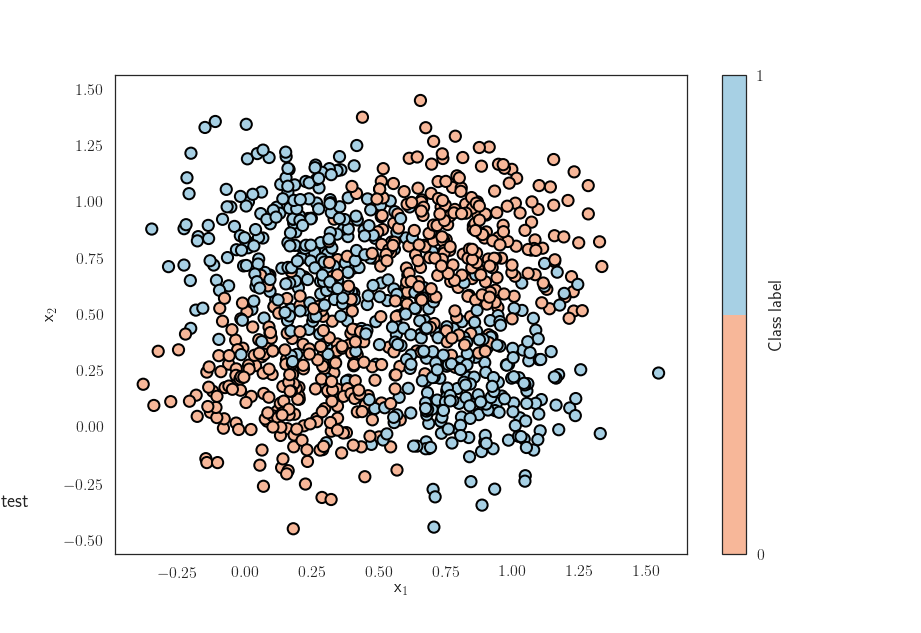
\includegraphics{Figures/21.png}
	    \caption{test, aklfajkldfjlakdfjklafljk}
		\label{fig:1}
	\end{figure}

\ref{fig:1}

    Explain why log. regression is a good approach for this data set

    \subsection{2.2}\label{section}

    \begin{Verbatim}[commandchars=\\\{\}]
{\color{incolor}In [{\color{incolor}7}]:} \PY{n}{w0} \PY{o}{=} \PY{n}{np}\PY{o}{.}\PY{n}{array}\PY{p}{(}\PY{p}{[}\PY{l+m+mi}{0}\PY{p}{,}\PY{l+m+mi}{0}\PY{p}{,}\PY{l+m+mi}{0}\PY{p}{]}\PY{p}{)}
        \PY{n}{phi} \PY{o}{=} \PY{n}{np}\PY{o}{.}\PY{n}{hstack}\PY{p}{(}\PY{p}{(}\PY{n}{np}\PY{o}{.}\PY{n}{ones}\PY{p}{(} \PY{p}{(}\PY{n}{x}\PY{o}{.}\PY{n}{shape}\PY{p}{[}\PY{l+m+mi}{0}\PY{p}{]}\PY{p}{,}\PY{l+m+mi}{1}\PY{p}{)} \PY{p}{)} \PY{p}{,}  \PY{n}{x}\PY{p}{)}\PY{p}{)}\PY{o}{.}\PY{n}{T}
        \PY{n}{w}\PY{p}{,} \PY{n}{i} \PY{o}{=} \PY{n}{RLS}\PY{p}{(}\PY{n}{x}\PY{p}{,} \PY{n}{c}\PY{p}{,} \PY{n}{phi}\PY{o}{.}\PY{n}{T}\PY{p}{,} \PY{n}{w0}\PY{p}{)}
        
        \PY{c+c1}{\PYZsh{} sigmoid function}
        \PY{c+c1}{\PYZsh{} probability before optimization}
        \PY{n}{prob\PYZus{}classified\PYZus{}before\PYZus{}opt} \PY{o}{=} \PY{n}{sigmoid}\PY{p}{(}\PY{n}{w0}\PY{o}{.}\PY{n}{dot}\PY{p}{(}\PY{n}{phi}\PY{p}{)}\PY{p}{)}
        \PY{n}{prob\PYZus{}classified\PYZus{}after\PYZus{}opt}  \PY{o}{=} \PY{n}{sigmoid}\PY{p}{(}\PY{n}{w}\PY{o}{.}\PY{n}{dot}\PY{p}{(}\PY{n}{phi}\PY{p}{)}\PY{p}{)}
        \PY{n}{c1} \PY{o}{=} \PY{n}{np}\PY{o}{.}\PY{n}{mean}\PY{p}{(}\PY{n}{prob\PYZus{}classified\PYZus{}after\PYZus{}opt}\PY{p}{[}\PY{n}{c} \PY{o}{==} \PY{l+m+mi}{1}\PY{p}{]}\PY{p}{)}
        \PY{n}{c2} \PY{o}{=} \PY{l+m+mi}{1} \PY{o}{\PYZhy{}} \PY{n}{c1}
        \PY{n+nb}{print}\PY{p}{(}\PY{p}{(}\PY{l+s+s1}{\PYZsq{}}\PY{l+s+s1}{The class probabilities are :}\PY{l+s+s1}{\PYZsq{}}\PYZbs{}
               \PY{l+s+s1}{\PYZsq{}}\PY{l+s+s1}{ class 1 = }\PY{l+s+si}{\PYZob{}0\PYZcb{}}\PY{l+s+s1}{, class 2 = }\PY{l+s+si}{\PYZob{}1\PYZcb{}}\PY{l+s+s1}{\PYZsq{}}\PY{p}{)}\PY{o}{.}\PYZbs{}
              \PY{n+nb}{format}\PY{p}{(}\PY{n}{c1}\PY{p}{,} \PY{l+m+mi}{1}\PY{o}{\PYZhy{}}\PY{n}{c1}\PY{p}{)}\PY{p}{)}
        
        \PY{n+nb}{print}\PY{p}{(}\PY{l+s+s1}{\PYZsq{}}\PY{l+s+s1}{w0 = }\PY{l+s+si}{\PYZob{}0\PYZcb{}}\PY{l+s+s1}{, i = }\PY{l+s+si}{\PYZob{}1\PYZcb{}}\PY{l+s+s1}{\PYZsq{}}\PY{o}{.}\PY{n}{format}\PY{p}{(}\PY{n}{w}\PY{p}{,} \PY{n}{i}\PY{p}{)}\PY{p}{)}
\end{Verbatim}

    \begin{Verbatim}[commandchars=\\\{\}]
The class probabilities are : class 1 = 0.49205021284958317, class 2 = 0.5079497871504168
w0 = [ 0.00440664 -0.02139153 -0.04930069], i = 3

    \end{Verbatim}

    \begin{Verbatim}[commandchars=\\\{\}]
{\color{incolor}In [{\color{incolor}8}]:} \PY{c+c1}{\PYZsh{} create feature matrix with bias}
        \PY{n}{tmp} \PY{o}{=} \PY{n}{np}\PY{o}{.}\PY{n}{ones}\PY{p}{(}\PY{p}{(}\PY{l+m+mi}{1}\PY{p}{,} \PY{n}{x}\PY{o}{.}\PY{n}{shape}\PY{p}{[}\PY{l+m+mi}{0}\PY{p}{]}\PY{p}{)}\PY{p}{)}
        \PY{n}{phi} \PY{o}{=} \PY{n}{np}\PY{o}{.}\PY{n}{vstack}\PY{p}{(}\PY{p}{[}\PY{n}{tmp}\PY{p}{,} \PY{n}{x}\PY{o}{.}\PY{n}{T}\PY{p}{]}\PY{p}{)}
        
        
        \PY{c+c1}{\PYZsh{} after optimization}
        \PY{n}{prob\PYZus{}classified\PYZus{}after\PYZus{}opt} \PY{o}{=}  \PY{n}{sigmoid}\PY{p}{(}\PY{n}{w}\PY{o}{.}\PY{n}{dot}\PY{p}{(}\PY{n}{phi}\PY{p}{)}\PY{p}{)}
        
        \PY{c+c1}{\PYZsh{} equation 4.90 Bisschop}
        \PY{n}{cross\PYZus{}entropy} \PY{o}{=} \PY{k}{lambda} \PY{n}{y}\PY{p}{,} \PY{n}{t}\PY{p}{:}\PYZbs{}
                \PY{o}{\PYZhy{}}\PY{n}{np}\PY{o}{.}\PY{n}{sum}\PY{p}{(} \PY{n}{t} \PY{o}{*} \PY{n}{np}\PY{o}{.}\PY{n}{log}\PY{p}{(}\PY{n}{y}\PY{p}{)} \PY{o}{+} \PY{p}{(}\PY{l+m+mi}{1} \PY{o}{\PYZhy{}} \PY{n}{t}\PY{p}{)} \PY{o}{*} \PY{n}{np}\PY{o}{.}\PY{n}{log}\PY{p}{(}\PY{l+m+mi}{1} \PY{o}{\PYZhy{}} \PY{n}{y}\PY{p}{)}\PY{p}{)}
        \PY{c+c1}{\PYZsh{} cross entropy with w = [0,0,0]}
        \PY{n}{cross\PYZus{}entropy\PYZus{}before\PYZus{}opt} \PY{o}{=} \PY{n}{cross\PYZus{}entropy}\PY{p}{(}\PY{n}{prob\PYZus{}classified\PYZus{}before\PYZus{}opt}\PY{p}{,} \PY{n}{c}\PY{p}{)}
        
        \PY{c+c1}{\PYZsh{} cross entropy after optimization using IRS}
        \PY{n}{cross\PYZus{}entropy\PYZus{}after\PYZus{}opt}  \PY{o}{=} \PY{n}{cross\PYZus{}entropy}\PY{p}{(}\PY{n}{prob\PYZus{}classified\PYZus{}after\PYZus{}opt}\PY{p}{,} \PY{n}{c}\PY{p}{)}
        \PY{n+nb}{print}\PY{p}{(}\PY{l+s+s1}{\PYZsq{}}\PY{l+s+s1}{cross\PYZhy{}entropy : before = }\PY{l+s+si}{\PYZob{}0\PYZcb{}}\PY{l+s+s1}{, after = }\PY{l+s+si}{\PYZob{}1\PYZcb{}}\PY{l+s+s1}{ optimization}\PY{l+s+s1}{\PYZsq{}}\PYZbs{}
              \PY{o}{.}\PY{n}{format}\PY{p}{(}\PY{n}{cross\PYZus{}entropy\PYZus{}before\PYZus{}opt}\PY{p}{,} \PY{n}{cross\PYZus{}entropy\PYZus{}after\PYZus{}opt}\PY{p}{)}\PY{p}{)}
        
        \PY{c+c1}{\PYZsh{} plot before optimization}
        \PY{n}{fig} \PY{o}{=} \PY{n}{figure}\PY{p}{(}\PY{p}{)}\PY{p}{;} \PY{n}{fig}\PY{o}{.}\PY{n}{clf}\PY{p}{(}\PY{p}{)}
        \PY{n}{ax} \PY{o}{=} \PY{n}{fig}\PY{o}{.}\PY{n}{add\PYZus{}subplot}\PY{p}{(}\PY{l+m+mi}{2}\PY{p}{,}\PY{l+m+mi}{1}\PY{p}{,}\PY{l+m+mi}{1}\PY{p}{)}
        \PY{n}{p} \PY{o}{=} \PY{n}{ax}\PY{o}{.}\PY{n}{scatter}\PY{p}{(}\PY{n}{x}\PY{p}{[}\PY{p}{:}\PY{p}{,}\PY{l+m+mi}{0}\PY{p}{]}\PY{p}{,} \PY{n}{x}\PY{p}{[}\PY{p}{:}\PY{p}{,}\PY{l+m+mi}{1}\PY{p}{]}\PY{p}{,} \PY{n}{c} \PY{o}{=} \PY{n}{prob\PYZus{}classified\PYZus{}before\PYZus{}opt}\PY{p}{,} \PY{n}{cmap} \PY{o}{=} \PY{n}{cmap\PYZus{}prob}\PY{p}{)}\PY{p}{;}
        \PY{n}{cb} \PY{o}{=} \PY{n}{fig}\PY{o}{.}\PY{n}{colorbar}\PY{p}{(}\PY{n}{p}\PY{p}{)}\PY{p}{;} \PY{n}{cb}\PY{o}{.}\PY{n}{set\PYZus{}label}\PY{p}{(}\PY{l+s+s1}{\PYZsq{}}\PY{l+s+s1}{p(\PYZdl{}c\PYZus{}1 }\PY{l+s+s1}{\PYZbs{}}\PY{l+s+s1}{mid }\PY{l+s+s1}{\PYZbs{}}\PY{l+s+s1}{phi\PYZdl{})}\PY{l+s+s1}{\PYZsq{}}\PY{p}{)}
        \PY{n}{ax}\PY{o}{.}\PY{n}{set\PYZus{}xlabel}\PY{p}{(}\PY{l+s+s1}{\PYZsq{}}\PY{l+s+s1}{x\PYZus{}1}\PY{l+s+s1}{\PYZsq{}}\PY{p}{)}
        \PY{n}{ax}\PY{o}{.}\PY{n}{set\PYZus{}ylabel}\PY{p}{(}\PY{l+s+s1}{\PYZsq{}}\PY{l+s+s1}{x\PYZus{}2}\PY{l+s+s1}{\PYZsq{}}\PY{p}{)}
        \PY{n}{sb}\PY{o}{.}\PY{n}{set\PYZus{}context}\PY{p}{(}\PY{l+s+s1}{\PYZsq{}}\PY{l+s+s1}{poster}\PY{l+s+s1}{\PYZsq{}}\PY{p}{)}
        \PY{n}{ax}\PY{o}{.}\PY{n}{set\PYZus{}title}\PY{p}{(}\PY{l+s+s1}{\PYZsq{}}\PY{l+s+s1}{Before optimization}\PY{l+s+s1}{\PYZsq{}}\PY{p}{)}
        
        \PY{c+c1}{\PYZsh{} plot after optimization}
        \PY{n}{ax} \PY{o}{=} \PY{n}{fig}\PY{o}{.}\PY{n}{add\PYZus{}subplot}\PY{p}{(}\PY{l+m+mi}{2}\PY{p}{,}\PY{l+m+mi}{1}\PY{p}{,}\PY{l+m+mi}{2}\PY{p}{)}
        \PY{n}{p} \PY{o}{=} \PY{n}{ax}\PY{o}{.}\PY{n}{scatter}\PY{p}{(}\PY{n}{x}\PY{p}{[}\PY{p}{:}\PY{p}{,}\PY{l+m+mi}{0}\PY{p}{]}\PY{p}{,} \PY{n}{x}\PY{p}{[}\PY{p}{:}\PY{p}{,}\PY{l+m+mi}{1}\PY{p}{]}\PY{p}{,} \PY{n}{c} \PY{o}{=} \PY{n}{prob\PYZus{}classified\PYZus{}after\PYZus{}opt}\PY{p}{,} \PY{n}{cmap} \PY{o}{=} \PY{n}{cmap\PYZus{}prob}\PY{p}{)}\PY{p}{;}
        \PY{n}{cb} \PY{o}{=} \PY{n}{fig}\PY{o}{.}\PY{n}{colorbar}\PY{p}{(}\PY{n}{p}\PY{p}{)}\PY{p}{;} \PY{n}{cb}\PY{o}{.}\PY{n}{set\PYZus{}label}\PY{p}{(}\PY{l+s+s1}{\PYZsq{}}\PY{l+s+s1}{p(\PYZdl{}c\PYZus{}1 }\PY{l+s+s1}{\PYZbs{}}\PY{l+s+s1}{mid }\PY{l+s+s1}{\PYZbs{}}\PY{l+s+s1}{phi\PYZdl{})}\PY{l+s+s1}{\PYZsq{}}\PY{p}{)}
        \PY{n}{ax}\PY{o}{.}\PY{n}{set\PYZus{}xlabel}\PY{p}{(}\PY{l+s+s1}{\PYZsq{}}\PY{l+s+s1}{x\PYZus{}1}\PY{l+s+s1}{\PYZsq{}}\PY{p}{)}
        \PY{n}{ax}\PY{o}{.}\PY{n}{set\PYZus{}ylabel}\PY{p}{(}\PY{l+s+s1}{\PYZsq{}}\PY{l+s+s1}{x\PYZus{}2}\PY{l+s+s1}{\PYZsq{}}\PY{p}{)}
        \PY{n}{sb}\PY{o}{.}\PY{n}{set\PYZus{}context}\PY{p}{(}\PY{l+s+s1}{\PYZsq{}}\PY{l+s+s1}{poster}\PY{l+s+s1}{\PYZsq{}}\PY{p}{)}
        \PY{n}{ax}\PY{o}{.}\PY{n}{set\PYZus{}title}\PY{p}{(}\PY{l+s+s1}{\PYZsq{}}\PY{l+s+s1}{After optimization}\PY{l+s+s1}{\PYZsq{}}\PY{p}{)}
        
        \PY{n}{fig}\PY{o}{.}\PY{n}{tight\PYZus{}layout}\PY{p}{(}\PY{p}{)}
        \PY{n}{savefig}\PY{p}{(}\PY{l+s+s1}{\PYZsq{}}\PY{l+s+s1}{Figures/22.png}\PY{l+s+s1}{\PYZsq{}}\PY{p}{)}
\end{Verbatim}

    \begin{Verbatim}[commandchars=\\\{\}]
cross-entropy : before = 693.1471805599454, after = 692.969359482537 optimization

    \end{Verbatim}

    \begin{Verbatim}[commandchars=\\\{\}]
{\color{incolor}In [{\color{incolor}9}]:} \PY{k+kn}{from} \PY{n+nn}{scipy}\PY{n+nn}{.}\PY{n+nn}{stats} \PY{k}{import} \PY{n}{multivariate\PYZus{}normal} \PY{k}{as} \PY{n}{mv}
        \PY{n}{create\PYZus{}basis\PYZus{}vector} \PY{o}{=} \PY{k}{lambda} \PY{n}{mu}\PY{p}{,} \PY{n}{sigma}\PY{p}{:} \PY{n}{mv}\PY{p}{(}\PY{n}{mu}\PY{p}{,} \PY{n}{sigma}\PY{p}{)}
        \PY{n}{mu1} \PY{o}{=} \PY{n}{np}\PY{o}{.}\PY{n}{array}\PY{p}{(}\PY{p}{[}\PY{l+m+mi}{0}\PY{p}{,}\PY{l+m+mi}{0}\PY{p}{]}\PY{p}{)}\PY{p}{;} \PY{n}{mu2} \PY{o}{=} \PY{n}{np}\PY{o}{.}\PY{n}{array}\PY{p}{(}\PY{p}{[}\PY{l+m+mi}{1}\PY{p}{,}\PY{l+m+mi}{1}\PY{p}{]}\PY{p}{)}
        \PY{n}{sigma2} \PY{o}{=} \PY{o}{.}\PY{l+m+mi}{2}
        
        \PY{n}{phi1} \PY{o}{=} \PY{n}{create\PYZus{}basis\PYZus{}vector}\PY{p}{(}\PY{n}{mu1}\PY{p}{,} \PY{n}{sigma2} \PY{o}{*} \PY{n}{np}\PY{o}{.}\PY{n}{eye}\PY{p}{(}\PY{l+m+mi}{2}\PY{p}{)}\PY{p}{)}
        \PY{n}{phi2} \PY{o}{=} \PY{n}{create\PYZus{}basis\PYZus{}vector}\PY{p}{(}\PY{n}{mu2}\PY{p}{,} \PY{n}{sigma2} \PY{o}{*} \PY{n}{np}\PY{o}{.}\PY{n}{eye}\PY{p}{(}\PY{l+m+mi}{2}\PY{p}{)}\PY{p}{)}
        
        \PY{n}{phi1\PYZus{}pdf} \PY{o}{=} \PY{n}{phi1}\PY{o}{.}\PY{n}{pdf}\PY{p}{(}\PY{n}{x}\PY{p}{)}\PY{p}{;}
        \PY{n}{phi2\PYZus{}pdf} \PY{o}{=} \PY{n}{phi2}\PY{o}{.}\PY{n}{pdf}\PY{p}{(}\PY{n}{x}\PY{p}{)}\PY{p}{;}
        
        \PY{n}{phi} \PY{o}{=}  \PY{n}{np}\PY{o}{.}\PY{n}{vstack}\PY{p}{(}\PY{p}{(}\PY{n}{np}\PY{o}{.}\PY{n}{ones}\PY{p}{(}\PY{n}{phi1\PYZus{}pdf}\PY{o}{.}\PY{n}{shape}\PY{p}{)}\PY{p}{,} \PY{n}{phi1\PYZus{}pdf}\PY{p}{,} \PY{n}{phi2\PYZus{}pdf}\PY{p}{)}\PY{p}{)}
        \PY{c+c1}{\PYZsh{} print(phi.shape, phi1\PYZus{}pdf.shape); assert 0}
        \PY{n}{w}\PY{p}{,} \PY{n}{i}  \PY{o}{=} \PY{n}{RLS}\PY{p}{(}\PY{n}{x}\PY{p}{,} \PY{n}{c}\PY{p}{,} \PY{n}{phi}\PY{o}{.}\PY{n}{T}\PY{p}{,} \PY{n}{w0}\PY{p}{)}
        
        
        \PY{n}{prob\PYZus{}gaussian\PYZus{}after\PYZus{}opt} \PY{o}{=} \PY{n}{sigmoid}\PY{p}{(}\PY{n}{w}\PY{o}{.}\PY{n}{dot}\PY{p}{(}\PY{n}{phi}\PY{p}{)}\PY{p}{)}
        \PY{n}{cross\PYZus{}entropy\PYZus{}gaussian} \PY{o}{=} \PY{n}{cross\PYZus{}entropy}\PY{p}{(}\PY{n}{prob\PYZus{}gaussian\PYZus{}after\PYZus{}opt}\PY{p}{,} \PY{n}{c}\PY{p}{)}
        \PY{n+nb}{print}\PY{p}{(}\PY{l+s+s1}{\PYZsq{}}\PY{l+s+s1}{Cross\PYZhy{}entropy with gaussian basis function = }\PY{l+s+si}{\PYZob{}0\PYZcb{}}\PY{l+s+s1}{\PYZsq{}}\PYZbs{}
             \PY{o}{.}\PY{n}{format}\PY{p}{(}\PY{n}{cross\PYZus{}entropy\PYZus{}gaussian}\PY{p}{)}\PY{p}{)}
        
        \PY{n}{fig} \PY{o}{=} \PY{n}{figure}\PY{p}{(}\PY{p}{)}
        \PY{c+c1}{\PYZsh{} subplot: origingal inputspace}
        \PY{n}{ax} \PY{o}{=} \PY{n}{fig}\PY{o}{.}\PY{n}{add\PYZus{}subplot}\PY{p}{(}\PY{l+m+mi}{211}\PY{p}{)}
        \PY{n}{p} \PY{o}{=} \PY{n}{ax}\PY{o}{.}\PY{n}{scatter}\PY{p}{(}\PY{n}{x}\PY{p}{[}\PY{p}{:}\PY{p}{,}\PY{l+m+mi}{0}\PY{p}{]}\PY{p}{,} \PY{n}{x}\PY{p}{[}\PY{p}{:}\PY{p}{,}\PY{l+m+mi}{1}\PY{p}{]}\PY{p}{,} \PYZbs{}
                       \PY{n}{c} \PY{o}{=} \PY{n}{c}\PY{p}{,} \PY{n}{cmap} \PY{o}{=} \PY{n}{cmap\PYZus{}class}\PY{p}{)}\PY{p}{;}
        \PY{n}{cb} \PY{o}{=} \PY{n}{fig}\PY{o}{.}\PY{n}{colorbar}\PY{p}{(}\PY{n}{p}\PY{p}{)}\PY{p}{;} \PY{n}{cb}\PY{o}{.}\PY{n}{set\PYZus{}label}\PY{p}{(}\PY{l+s+s1}{\PYZsq{}}\PY{l+s+s1}{Class label}\PY{l+s+s1}{\PYZsq{}}\PY{p}{)}
        \PY{n}{ax}\PY{o}{.}\PY{n}{set\PYZus{}title}\PY{p}{(}\PY{l+s+s1}{\PYZsq{}}\PY{l+s+s1}{Original input space}\PY{l+s+s1}{\PYZsq{}}\PY{p}{)}
        \PY{n}{ax}\PY{o}{.}\PY{n}{set\PYZus{}xlabel}\PY{p}{(}\PY{l+s+s1}{\PYZsq{}}\PY{l+s+s1}{\PYZdl{}x\PYZus{}1\PYZdl{}}\PY{l+s+s1}{\PYZsq{}}\PY{p}{)}
        \PY{n}{ax}\PY{o}{.}\PY{n}{set\PYZus{}ylabel}\PY{p}{(}\PY{l+s+s1}{\PYZsq{}}\PY{l+s+s1}{\PYZdl{}x\PYZus{}2\PYZdl{}}\PY{l+s+s1}{\PYZsq{}}\PY{p}{)}
        
        \PY{c+c1}{\PYZsh{} basis function decomposition}
        \PY{n}{ax} \PY{o}{=} \PY{n}{fig}\PY{o}{.}\PY{n}{add\PYZus{}subplot}\PY{p}{(}\PY{l+m+mi}{212}\PY{p}{)}
        \PY{n}{ax}\PY{o}{.}\PY{n}{set\PYZus{}xlabel}\PY{p}{(}\PY{l+s+s1}{\PYZsq{}}\PY{l+s+s1}{\PYZdl{}x\PYZus{}1\PYZdl{}}\PY{l+s+s1}{\PYZsq{}}\PY{p}{)}
        \PY{n}{ax}\PY{o}{.}\PY{n}{set\PYZus{}ylabel}\PY{p}{(}\PY{l+s+s1}{\PYZsq{}}\PY{l+s+s1}{\PYZdl{}x\PYZus{}2\PYZdl{}}\PY{l+s+s1}{\PYZsq{}}\PY{p}{)}
        \PY{n}{sb}\PY{o}{.}\PY{n}{set\PYZus{}context}\PY{p}{(}\PY{l+s+s1}{\PYZsq{}}\PY{l+s+s1}{poster}\PY{l+s+s1}{\PYZsq{}}\PY{p}{)}
        
        \PY{n}{p} \PY{o}{=} \PY{n}{ax}\PY{o}{.}\PY{n}{scatter}\PY{p}{(}\PY{n}{phi1}\PY{o}{.}\PY{n}{pdf}\PY{p}{(}\PY{n}{x}\PY{p}{)}\PY{p}{,} \PY{n}{phi2}\PY{o}{.}\PY{n}{pdf}\PY{p}{(}\PY{n}{x}\PY{p}{)}\PY{p}{,} \PYZbs{}
                       \PY{n}{c} \PY{o}{=} \PY{n}{c}\PY{p}{,} \PY{n}{cmap} \PY{o}{=} \PY{n}{cmap\PYZus{}class}\PY{p}{)}\PY{p}{;}
        \PY{n}{cb} \PY{o}{=} \PY{n}{fig}\PY{o}{.}\PY{n}{colorbar}\PY{p}{(}\PY{n}{p}\PY{p}{)}\PY{p}{;} \PY{n}{cb}\PY{o}{.}\PY{n}{set\PYZus{}label}\PY{p}{(}\PY{l+s+s1}{\PYZsq{}}\PY{l+s+s1}{Class label}\PY{l+s+s1}{\PYZsq{}}\PY{p}{)}
        
        \PY{n}{ax}\PY{o}{.}\PY{n}{set\PYZus{}xlabel}\PY{p}{(}\PY{l+s+s1}{\PYZsq{}}\PY{l+s+s1}{\PYZdl{}}\PY{l+s+s1}{\PYZbs{}}\PY{l+s+s1}{phi\PYZus{}1\PYZdl{}}\PY{l+s+s1}{\PYZsq{}}\PY{p}{)}
        \PY{n}{ax}\PY{o}{.}\PY{n}{set\PYZus{}ylabel}\PY{p}{(}\PY{l+s+s1}{\PYZsq{}}\PY{l+s+s1}{\PYZdl{}}\PY{l+s+s1}{\PYZbs{}}\PY{l+s+s1}{phi\PYZus{}2\PYZdl{}}\PY{l+s+s1}{\PYZsq{}}\PY{p}{)}
        \PY{n}{ax}\PY{o}{.}\PY{n}{set\PYZus{}title}\PY{p}{(}\PY{l+s+s1}{\PYZsq{}}\PY{l+s+s1}{basis vector space}\PY{l+s+s1}{\PYZsq{}}\PY{p}{)}
        \PY{n}{sb}\PY{o}{.}\PY{n}{set\PYZus{}context}\PY{p}{(}\PY{l+s+s1}{\PYZsq{}}\PY{l+s+s1}{poster}\PY{l+s+s1}{\PYZsq{}}\PY{p}{)}
        \PY{n}{fig}\PY{o}{.}\PY{n}{tight\PYZus{}layout}\PY{p}{(}\PY{p}{)}
        \PY{n}{savefig}\PY{p}{(}\PY{l+s+s1}{\PYZsq{}}\PY{l+s+s1}{Figures/24.png}\PY{l+s+s1}{\PYZsq{}}\PY{p}{)}
\end{Verbatim}

    \begin{Verbatim}[commandchars=\\\{\}]
Cross-entropy with gaussian basis function = 346.50408046148465

    \end{Verbatim}

    \begin{Verbatim}[commandchars=\\\{\}]
{\color{incolor}In [{\color{incolor}10}]:} \PY{n}{fig} \PY{o}{=} \PY{n}{figure}\PY{p}{(}\PY{p}{)}
         
         \PY{c+c1}{\PYZsh{} optimization results using basis functions}
         \PY{n}{ax} \PY{o}{=} \PY{n}{fig}\PY{o}{.}\PY{n}{add\PYZus{}subplot}\PY{p}{(}\PY{l+m+mi}{211}\PY{p}{)}
         \PY{n}{p} \PY{o}{=} \PY{n}{ax}\PY{o}{.}\PY{n}{scatter}\PY{p}{(}\PY{n}{phi1}\PY{o}{.}\PY{n}{pdf}\PY{p}{(}\PY{n}{x}\PY{p}{)}\PY{p}{,} \PY{n}{phi2}\PY{o}{.}\PY{n}{pdf}\PY{p}{(}\PY{n}{x}\PY{p}{)}\PY{p}{,}\PYZbs{}
            \PY{n}{c} \PY{o}{=} \PY{n}{prob\PYZus{}gaussian\PYZus{}after\PYZus{}opt} \PY{p}{,}\PYZbs{}
                        \PY{n}{cmap} \PY{o}{=} \PY{n}{cmap\PYZus{}prob}\PY{p}{)}\PY{p}{;}
         \PY{n}{cb} \PY{o}{=} \PY{n}{fig}\PY{o}{.}\PY{n}{colorbar}\PY{p}{(}\PY{n}{p}\PY{p}{)}\PY{p}{;} \PY{n}{cb}\PY{o}{.}\PY{n}{set\PYZus{}label}\PY{p}{(}\PY{l+s+s1}{\PYZsq{}}\PY{l+s+s1}{p(\PYZdl{}c\PYZus{}1 }\PY{l+s+s1}{\PYZbs{}}\PY{l+s+s1}{mid t)\PYZdl{}}\PY{l+s+s1}{\PYZsq{}}\PY{p}{)}
         \PY{n}{ax}\PY{o}{.}\PY{n}{set\PYZus{}xlabel}\PY{p}{(}\PY{l+s+s1}{\PYZsq{}}\PY{l+s+s1}{\PYZdl{}}\PY{l+s+s1}{\PYZbs{}}\PY{l+s+s1}{phi\PYZus{}1\PYZdl{}}\PY{l+s+s1}{\PYZsq{}}\PY{p}{)}
         \PY{n}{ax}\PY{o}{.}\PY{n}{set\PYZus{}ylabel}\PY{p}{(}\PY{l+s+s1}{\PYZsq{}}\PY{l+s+s1}{\PYZdl{}}\PY{l+s+s1}{\PYZbs{}}\PY{l+s+s1}{phi\PYZus{}2\PYZdl{}}\PY{l+s+s1}{\PYZsq{}}\PY{p}{)}
         \PY{n}{ax}\PY{o}{.}\PY{n}{set\PYZus{}title}\PY{p}{(}\PY{l+s+s1}{\PYZsq{}}\PY{l+s+s1}{\PYZdl{}P(c\PYZus{}1 }\PY{l+s+s1}{\PYZbs{}}\PY{l+s+s1}{mid t)\PYZdl{} in basis  space}\PY{l+s+s1}{\PYZsq{}}\PY{p}{)}
         
         \PY{n}{ax} \PY{o}{=} \PY{n}{fig}\PY{o}{.}\PY{n}{add\PYZus{}subplot}\PY{p}{(}\PY{l+m+mi}{212}\PY{p}{)}
         \PY{n}{p} \PY{o}{=} \PY{n}{ax}\PY{o}{.}\PY{n}{scatter}\PY{p}{(}\PY{n}{x}\PY{p}{[}\PY{p}{:}\PY{p}{,}\PY{l+m+mi}{0}\PY{p}{]}\PY{p}{,} \PY{n}{x}\PY{p}{[}\PY{p}{:}\PY{p}{,}\PY{l+m+mi}{1}\PY{p}{]}\PY{p}{,}\PYZbs{}
            \PY{n}{c} \PY{o}{=} \PY{n}{prob\PYZus{}gaussian\PYZus{}after\PYZus{}opt} \PY{p}{,}\PYZbs{}
                        \PY{n}{cmap} \PY{o}{=} \PY{n}{cmap\PYZus{}prob}\PY{p}{)}\PY{p}{;}
         \PY{n}{cb} \PY{o}{=} \PY{n}{fig}\PY{o}{.}\PY{n}{colorbar}\PY{p}{(}\PY{n}{p}\PY{p}{)}\PY{p}{;} \PY{n}{cb}\PY{o}{.}\PY{n}{set\PYZus{}label}\PY{p}{(}\PY{l+s+s1}{\PYZsq{}}\PY{l+s+s1}{p(\PYZdl{}c\PYZus{}1 }\PY{l+s+s1}{\PYZbs{}}\PY{l+s+s1}{mid t)\PYZdl{}}\PY{l+s+s1}{\PYZsq{}}\PY{p}{)}
         
         \PY{n}{ax}\PY{o}{.}\PY{n}{set\PYZus{}xlabel}\PY{p}{(}\PY{l+s+s1}{\PYZsq{}}\PY{l+s+s1}{\PYZdl{}x\PYZus{}1\PYZdl{}}\PY{l+s+s1}{\PYZsq{}}\PY{p}{)}
         \PY{n}{ax}\PY{o}{.}\PY{n}{set\PYZus{}ylabel}\PY{p}{(}\PY{l+s+s1}{\PYZsq{}}\PY{l+s+s1}{\PYZdl{}x\PYZus{}2\PYZdl{}}\PY{l+s+s1}{\PYZsq{}}\PY{p}{)}
         \PY{n}{ax}\PY{o}{.}\PY{n}{set\PYZus{}title}\PY{p}{(}\PY{l+s+s1}{\PYZsq{}}\PY{l+s+s1}{\PYZdl{}P(c\PYZus{}1 }\PY{l+s+s1}{\PYZbs{}}\PY{l+s+s1}{mid t)\PYZdl{} in original space}\PY{l+s+s1}{\PYZsq{}}\PY{p}{)}
         \PY{n}{sb}\PY{o}{.}\PY{n}{set\PYZus{}context}\PY{p}{(}\PY{l+s+s1}{\PYZsq{}}\PY{l+s+s1}{poster}\PY{l+s+s1}{\PYZsq{}}\PY{p}{)}
         \PY{n}{fig}\PY{o}{.}\PY{n}{tight\PYZus{}layout}\PY{p}{(}\PY{p}{)}
         \PY{n}{savefig}\PY{p}{(}\PY{l+s+s1}{\PYZsq{}}\PY{l+s+s1}{Figures/24.png}\PY{l+s+s1}{\PYZsq{}}\PY{p}{)}
\end{Verbatim}


    % Add a bibliography block to the postdoc
    
    
    
    \end{document}
